
\begin{figure}
	\centering
	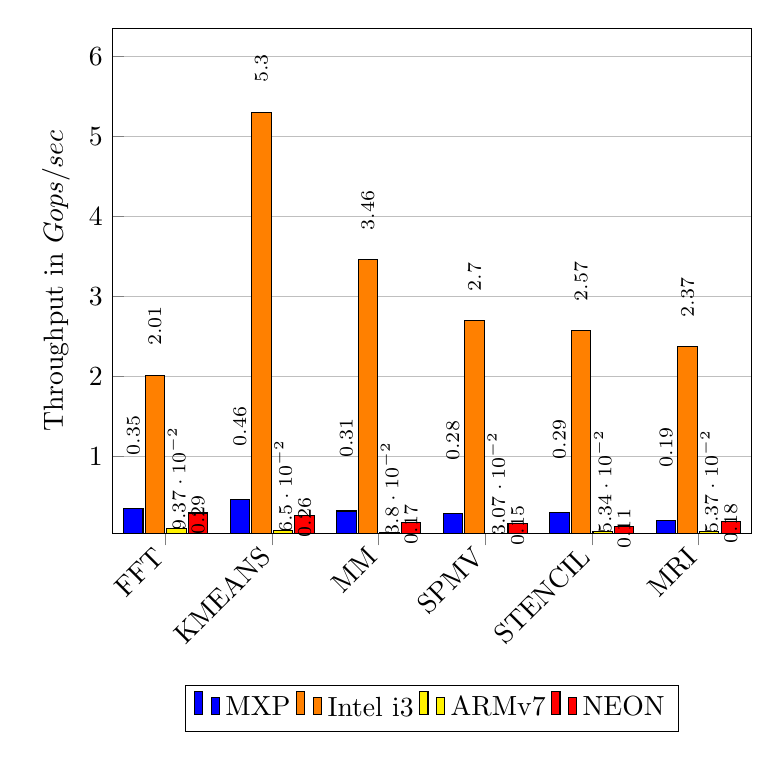
\begin{tikzpicture}
	\begin{axis}[
	width  = 0.8*\textwidth,
	height = 8cm,
	xtick pos=left,
	ytick pos=left,
%	major x tick style = transparent,
	x tick label style={rotate=45, anchor=east, align=right,text width=2cm},
	bar width=7pt,
	ymajorgrids = true,
	ylabel = {Throughput in $Gops/sec$},
	symbolic x coords={FFT,KMEANS,MM,SPMV,STENCIL,MRI},
	xtick = data,
	nodes near coords,
	ybar,
	every node near coord/.append style={rotate=90, anchor=west,font=\scriptsize, xshift=0.25cm},
	scaled y ticks = false,
	enlarge y limits={upper,value=0.2},
%	enlarge x limits=0.25,
	ybar=2*\pgflinewidth,
	legend cell align=left,
	legend style={
		at={(.5,-0.3)},
		anchor=north,
		legend columns=-1
		column sep=0.5ex
	}
	]
	\addplot[draw=black,fill=blue,every node near coord/.append style={xshift=.3cm}]
	coordinates {(FFT, 0.349) (KMEANS,0.457) (MM,0.313) (SPMV,0.2798) (STENCIL,0.294) (MRI,0.194)};
	
	\addplot[draw=black,fill=orange]
	coordinates  {(FFT, 2.01) (KMEANS,5.301) (MM,3.456) (SPMV,2.696) (STENCIL,2.57) (MRI,2.368)};
	
	\addplot[draw=black,fill=yellow,every node near coord/.append style={xshift=-0.4cm}]
	coordinates  {(FFT,0.0937) (KMEANS,0.065) (MM,0.038) (SPMV,0.0307) (STENCIL,0.0534) (MRI,0.0537)};
	
	\addplot[draw=black,fill=red,every node near coord/.append style={xshift=-0.65cm}]
	coordinates {(FFT, 0.2887) (KMEANS,0.257) (MM,0.165) (SPMV,0.1529) (STENCIL,0.1146) (MRI,0.1839)};
	
	\legend{MXP,Intel i3,ARMv7,NEON}
	\end{axis}
	\end{tikzpicture}
	\caption{Halfword(16-bits) level throughput(Gops/sec) for compute Kernels}
	\label{kernel:2}
\end{figure}